\documentclass[11pt]{utalcaDoc}
\usepackage{alltt}
\usepackage{underscore}
\usepackage[utf8]{inputenc}
\usepackage[activeacute,spanish]{babel}
\usepackage{verbatim}
\usepackage[pdftex]{graphicx}
\usepackage{ae}
\usepackage{amsmath}
\usepackage{amsfonts}
\usepackage{pdflscape}
\usepackage{inconsolata}
\usepackage{url}
\usepackage{hyperref}
\usepackage{listings}
% \usepackage{placeins}
\usepackage[section]{placeins}
\usepackage[stable]{footmisc}
\usepackage{minted}
\usepackage{multicol}

\usepackage{csquotes}
\title{{\bf Seguridad Informática}\\ Laboratorio 4}
\author{Erik Regla\\ eregla09@alumnos.utalca.cl}
\date{\today}

\begin{document}
\maketitle
\newpage
\tableofcontents
\newpage

\section{Actividades}
\subsection{Actividad 1}{Deberá entregar como actividad las capturas de pantalla del procedimiento de instalación y
de los resultados obtenidos.}

Ejecuté \texttt{docker pull wpscanteam/wpscan} ya que no instalé nada, solo ejecuto la imagen de docker~\cite{REF:wpscan}.


\begin{figure}[H]
	\centering
	\centering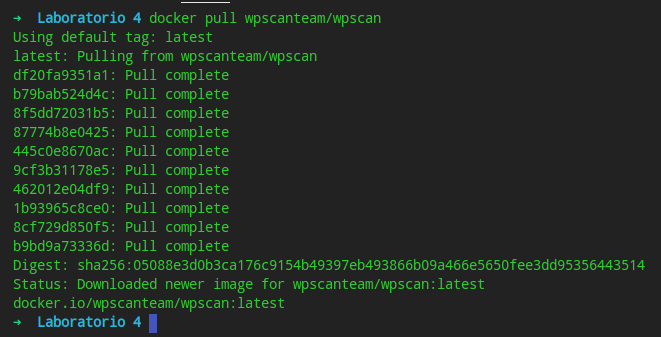
\includegraphics[width=.80\textwidth]{images/docker.png}
\caption{Resultado de cargar la imagen de docker.}
\label{FIG:docker}
\end{figure}

\subsection{Actividad 2}{Para esta actividad deberá buscar 3 sitios que se hayan montado utilizando wordpress. Para
esto deberá utilizar comandos de google hacking vistos en el laboratorio anterior.}

\begin{figure}[H]
	\centering
\begin{multicols}{3}
	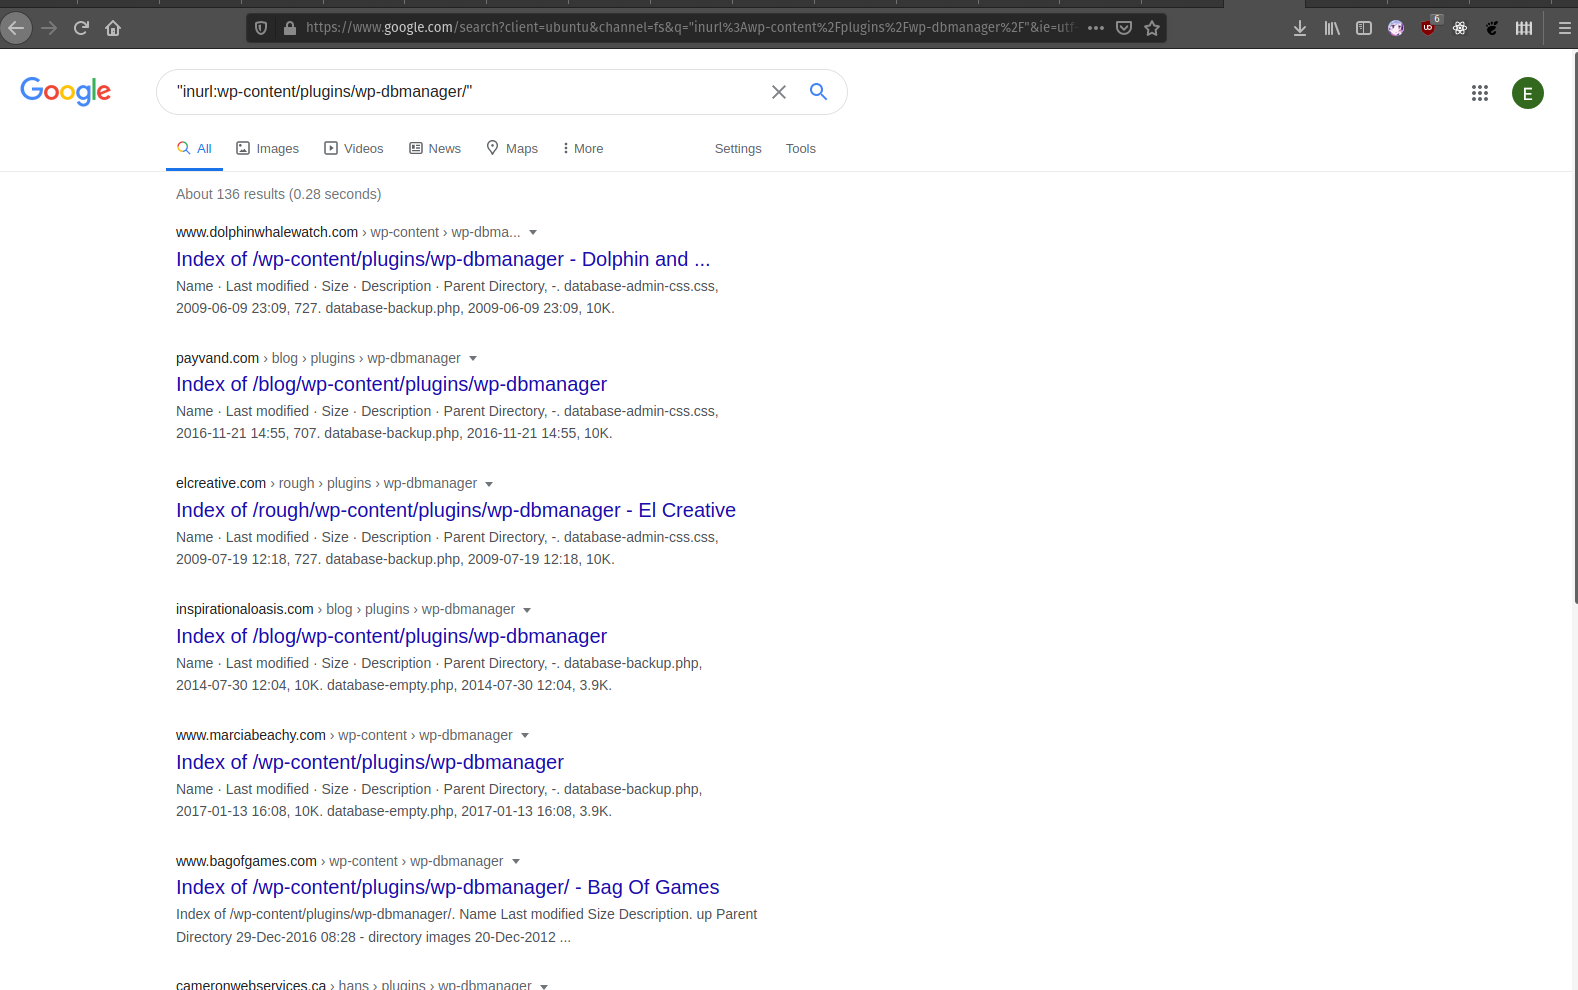
\includegraphics[width=.30\textwidth]{images/google1.png}\\
	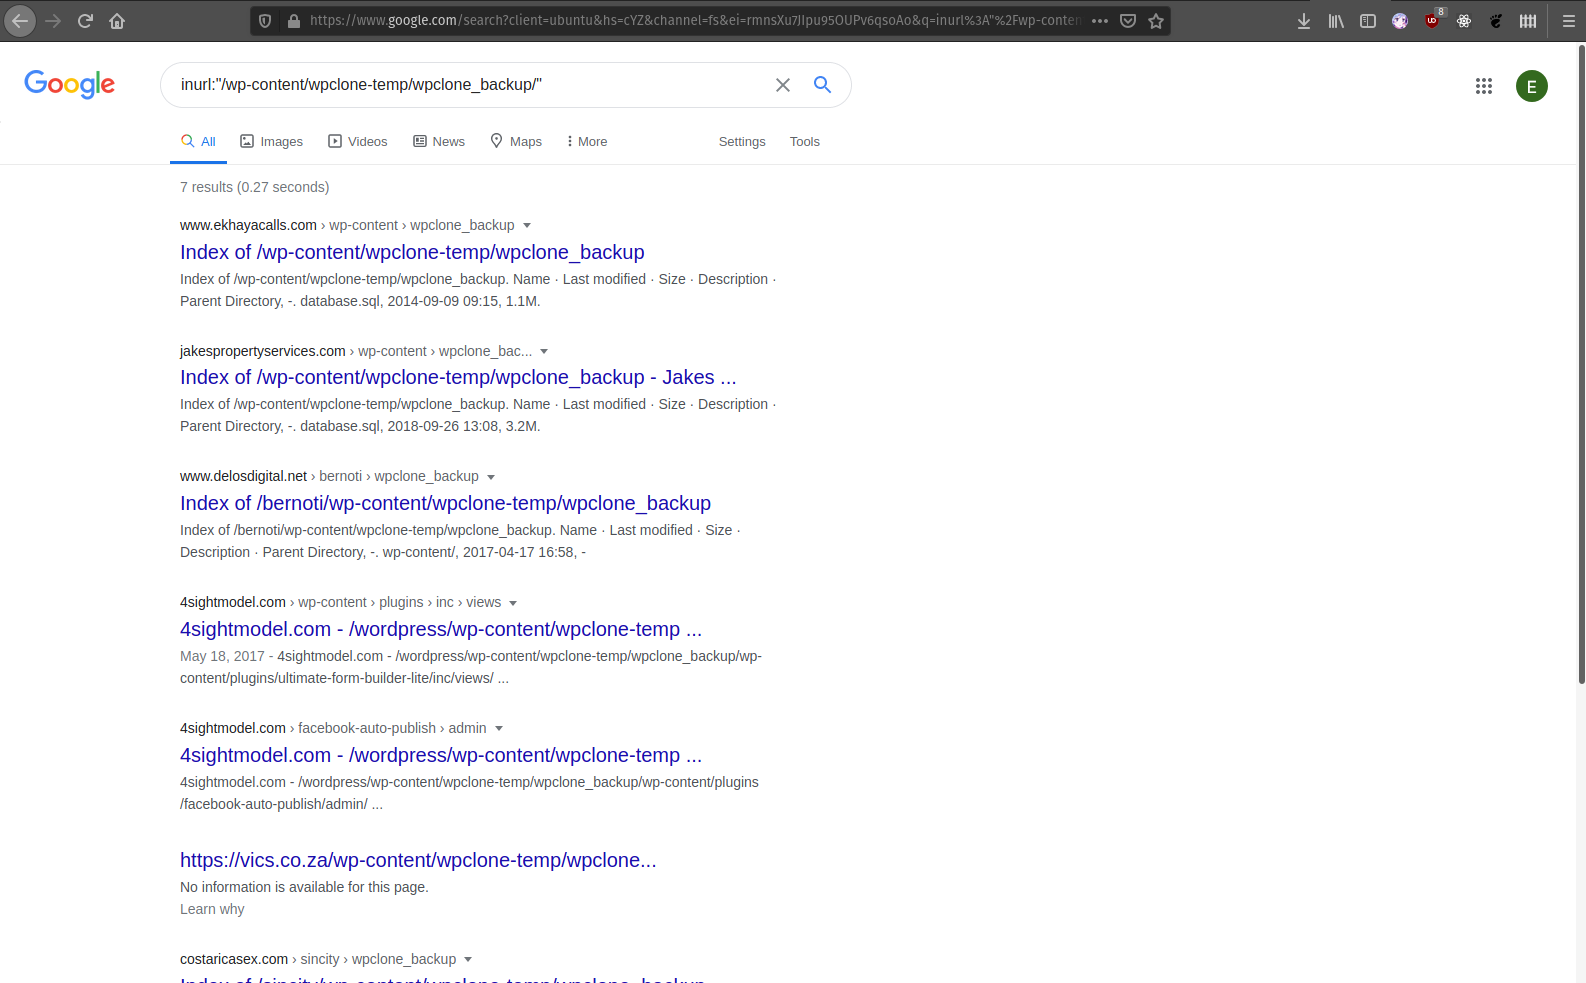
\includegraphics[width=.30\textwidth]{images/google2.png}\\
	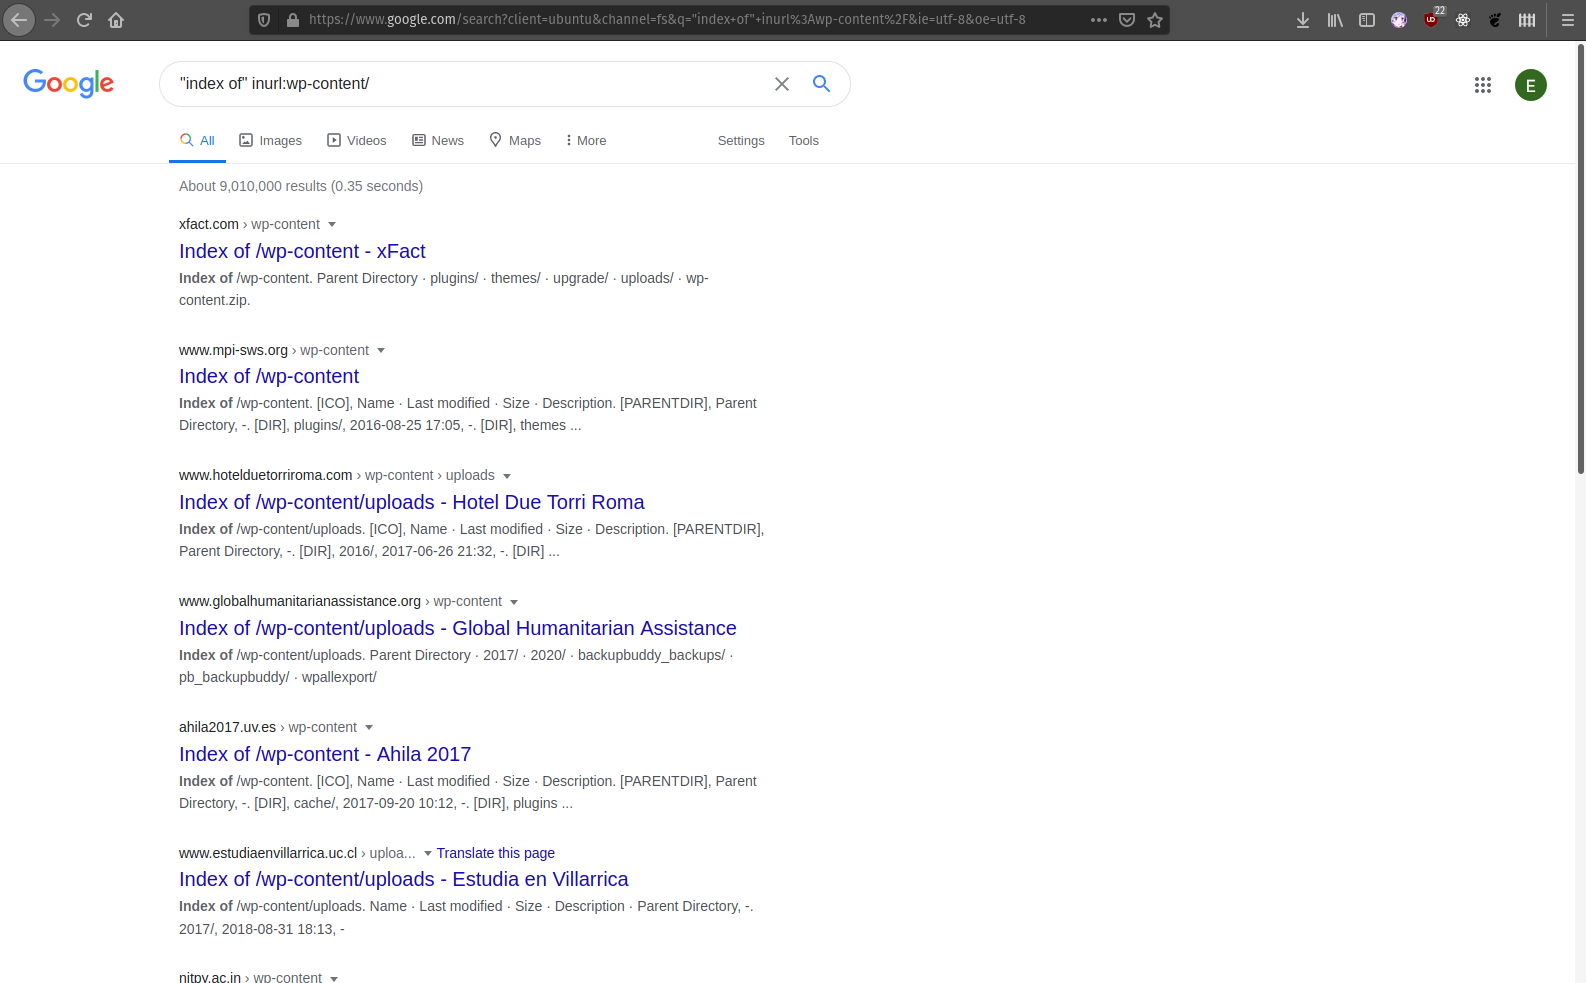
\includegraphics[width=.30\textwidth]{images/google3.png}\\
\end{multicols}
\caption{Comandos para google hacking}
\label{FIG:google}
\end{figure}

Los sitios elegidos son:
\begin{itemize}
	\item \texttt{https://www.mpi-sws.org/}
	\item \texttt{https://www.delosdigital.com/}
	\item \texttt{http://www.dolphinwhalewatch.com/}
\end{itemize}



\subsection{Actividad 3}{Para esta actividad deberá utilizar WPScan en los sitios encontrados en el punto anterior.
Para cada sitio escaneado con la herramienta deberá explicar las vulnerabilidades encontradas y
entregar recomendaciones de mitigación. Además deberá explicar como cree que afectan a las 3
propiedades principales de la Seguridad Informática (Confidencialidad, Integridad y Disponibilidad).}

\subsubsection{https://www.mpi-sws.org/}
\begin{minted}[linenos,tabsize=2,breaklines,fontsize=\scriptsize]{bash}
kuky_nekoi@fu-no-isan:~/.wpscan$ docker run -it --rm wpscanteam/wpscan --api-token DCTk3QgEgClCDCpU15LHbvxObvs6KnLij8SK3gsHcPM --url https://www.mpi-sws.org/  | egrep "(Title|WordPress version )"
[+] WordPress version 4.6 identified (Insecure, released on 2016-08-16).
 | [!] Title: WordPress 2.5-4.6 - Authenticated Stored Cross-Site Scripting via Image Filename
 | [!] Title: WordPress 2.8-4.6 - Path Traversal in Upgrade Package Uploader
 | [!] Title: WordPress 4.3-4.7 - Remote Code Execution (RCE) in PHPMailer
 | [!] Title: WordPress 2.9-4.7 - Authenticated Cross-Site scripting (XSS) in update-core.php
 | [!] Title: WordPress 3.4-4.7 - Stored Cross-Site Scripting (XSS) via Theme Name fallback
 | [!] Title: WordPress <= 4.7 - Post via Email Checks mail.example.com by Default
 | [!] Title: WordPress 2.8-4.7 - Accessibility Mode Cross-Site Request Forgery (CSRF)
 | [!] Title: WordPress 3.0-4.7 - Cryptographically Weak Pseudo-Random Number Generator (PRNG)
 | [!] Title: WordPress 4.2.0-4.7.1 - Press This UI Available to Unauthorised Users
 | [!] Title: WordPress 3.5-4.7.1 - WP_Query SQL Injection
 | [!] Title: WordPress 4.3.0-4.7.1 - Cross-Site Scripting (XSS) in posts list table
 | [!] Title: WordPress 3.6.0-4.7.2 - Authenticated Cross-Site Scripting (XSS) via Media File Metadata
 | [!] Title: WordPress 2.8.1-4.7.2 - Control Characters in Redirect URL Validation
 | [!] Title: WordPress  4.0-4.7.2 - Authenticated Stored Cross-Site Scripting (XSS) in YouTube URL Embeds
 | [!] Title: WordPress 4.2-4.7.2 - Press This CSRF DoS
 | [!] Title: WordPress 2.3-4.8.3 - Host Header Injection in Password Reset
 | [!] Title: WordPress 2.7.0-4.7.4 - Insufficient Redirect Validation
 | [!] Title: WordPress 2.5.0-4.7.4 - Post Meta Data Values Improper Handling in XML-RPC
 | [!] Title: WordPress 3.4.0-4.7.4 - XML-RPC Post Meta Data Lack of Capability Checks 
 | [!] Title: WordPress 2.5.0-4.7.4 - Filesystem Credentials Dialog CSRF
 | [!] Title: WordPress 3.3-4.7.4 - Large File Upload Error XSS
 | [!] Title: WordPress 3.4.0-4.7.4 - Customizer XSS & CSRF
 | [!] Title: WordPress 2.3.0-4.8.1 - $wpdb->prepare() potential SQL Injection
 | [!] Title: WordPress 2.3.0-4.7.4 - Authenticated SQL injection
 | [!] Title: WordPress 2.9.2-4.8.1 - Open Redirect
 | [!] Title: WordPress 3.0-4.8.1 - Path Traversal in Unzipping
 | [!] Title: WordPress 4.4-4.8.1 - Cross-Site Scripting (XSS) in oEmbed
 | [!] Title: WordPress 4.2.3-4.8.1 - Authenticated Cross-Site Scripting (XSS) in Visual Editor
 | [!] Title: WordPress <= 4.8.2 - $wpdb->prepare() Weakness
 | [!] Title: WordPress 2.8.6-4.9 - Authenticated JavaScript File Upload
 | [!] Title: WordPress 1.5.0-4.9 - RSS and Atom Feed Escaping
 | [!] Title: WordPress 4.3.0-4.9 - HTML Language Attribute Escaping
 | [!] Title: WordPress 3.7-4.9 - 'newbloguser' Key Weak Hashing
 | [!] Title: WordPress 3.7-4.9.1 - MediaElement Cross-Site Scripting (XSS)
 | [!] Title: WordPress <= 4.9.4 - Application Denial of Service (DoS) (unpatched)
 | [!] Title: WordPress 3.7-4.9.4 - Remove localhost Default
 | [!] Title: WordPress 3.7-4.9.4 - Use Safe Redirect for Login
 | [!] Title: WordPress 3.7-4.9.4 - Escape Version in Generator Tag
 | [!] Title: WordPress <= 4.9.6 - Authenticated Arbitrary File Deletion
 | [!] Title: WordPress <= 5.0 - Authenticated File Delete
 | [!] Title: WordPress <= 5.0 - Authenticated Post Type Bypass
 | [!] Title: WordPress <= 5.0 - PHP Object Injection via Meta Data
 | [!] Title: WordPress <= 5.0 - Authenticated Cross-Site Scripting (XSS)
 | [!] Title: WordPress <= 5.0 - Cross-Site Scripting (XSS) that could affect plugins
 | [!] Title: WordPress <= 5.0 - User Activation Screen Search Engine Indexing
 | [!] Title: WordPress <= 5.0 - File Upload to XSS on Apache Web Servers
 | [!] Title: WordPress 3.7-5.0 (except 4.9.9) - Authenticated Code Execution
 | [!] Title: WordPress 3.9-5.1 - Comment Cross-Site Scripting (XSS)
 | [!] Title: WordPress <= 5.2.2 - Cross-Site Scripting (XSS) in URL Sanitisation
 | [!] Title: WordPress <= 5.2.3 - Stored XSS in Customizer
 | [!] Title: WordPress <= 5.2.3 - Unauthenticated View Private/Draft Posts
 | [!] Title: WordPress <= 5.2.3 - Stored XSS in Style Tags
 | [!] Title: WordPress <= 5.2.3 - JSON Request Cache Poisoning
 | [!] Title: WordPress <= 5.2.3 - Server-Side Request Forgery (SSRF) in URL Validation 
 | [!] Title: WordPress <= 5.2.3 - Admin Referrer Validation
 | [!] Title: WordPress <= 5.3 - Authenticated Improper Access Controls in REST API
 | [!] Title: WordPress <= 5.3 - Authenticated Stored XSS via Crafted Links
 | [!] Title: WordPress <= 5.3 - Authenticated Stored XSS via Block Editor Content
 | [!] Title: WordPress <= 5.3 - wp_kses_bad_protocol() Colon Bypass
 | [!] Title: WordPress < 5.4.1 - Password Reset Tokens Failed to Be Properly Invalidated
 | [!] Title: WordPress < 5.4.1 - Unauthenticated Users View Private Posts
 | [!] Title: WordPress < 5.4.1 - Authenticated Cross-Site Scripting (XSS) in Customizer
 | [!] Title: WordPress < 5.4.1 - Cross-Site Scripting (XSS) in wp-object-cache
 | [!] Title: WordPress < 5.4.1 - Authenticated Cross-Site Scripting (XSS) in File Uploads
 | [!] Title: WordPress <= 5.2.3 - Hardening Bypass
 | [!] Title: WordPress < 5.4.2 - Authenticated XSS via Media Files
 | [!] Title: WordPress < 5.4.2 - Open Redirection
 | [!] Title: WordPress < 5.4.2 - Authenticated XSS via Theme Upload
 | [!] Title: WordPress < 5.4.2 - Misuse of set-screen-option Leading to Privilege Escalation
 | [!] Title: WordPress < 5.4.2 - Disclosure of Password-Protected Page/Post Comments
kuky_nekoi@fu-no-isan:~/.wpscan$ 
   kuky_nekoi@fu-no-isan:~/.wpscan$    
\end{minted}

Por economía de espacio se omitirán las mitigaciones individuales para este sitio ya que es necesario actualizarlo de manera urgente. Un sitio expuesto a inyecciones SQL pone en peligro las tres propiedades principales de la seguridad informática.


\subsubsection{https://www.delosdigital.com/}
\begin{minted}[linenos,tabsize=2,breaklines,fontsize=\scriptsize]{bash}
kuky_nekoi@fu-no-isan:~/.wpscan$ docker run -it --rm wpscanteam/wpscan --api-token DCTk3QgEgClCDCpU15LHbvxObvs6KnLij8SK3gsHcPM --url https://www.mpi-sws.org/ | egrep "(Title|WordPress version )"
[+] WordPress version 4.6 identified (Insecure, released on 2016-08-16).
	| [!] Title: WordPress 2.5-4.6 - Authenticated Stored Cross-Site Scripting via Image Filename
	| [!] Title: WordPress 2.8-4.6 - Path Traversal in Upgrade Package Uploader
	| [!] Title: WordPress 4.3-4.7 - Remote Code Execution (RCE) in PHPMailer
	| [!] Title: WordPress 2.9-4.7 - Authenticated Cross-Site scripting (XSS) in update-core.php
	| [!] Title: WordPress 3.4-4.7 - Stored Cross-Site Scripting (XSS) via Theme Name fallback
	| [!] Title: WordPress <= 4.7 - Post via Email Checks mail.example.com by Default
	| [!] Title: WordPress 2.8-4.7 - Accessibility Mode Cross-Site Request Forgery (CSRF)
	| [!] Title: WordPress 3.0-4.7 - Cryptographically Weak Pseudo-Random Number Generator (PRNG)
	| [!] Title: WordPress 4.2.0-4.7.1 - Press This UI Available to Unauthorised Users
	| [!] Title: WordPress 3.5-4.7.1 - WP_Query SQL Injection
	| [!] Title: WordPress 4.3.0-4.7.1 - Cross-Site Scripting (XSS) in posts list table
	| [!] Title: WordPress 3.6.0-4.7.2 - Authenticated Cross-Site Scripting (XSS) via Media File Metadata
	| [!] Title: WordPress 2.8.1-4.7.2 - Control Characters in Redirect URL Validation
	| [!] Title: WordPress  4.0-4.7.2 - Authenticated Stored Cross-Site Scripting (XSS) in YouTube URL Embeds
	| [!] Title: WordPress 4.2-4.7.2 - Press This CSRF DoS
	| [!] Title: WordPress 2.3-4.8.3 - Host Header Injection in Password Reset
	| [!] Title: WordPress 2.7.0-4.7.4 - Insufficient Redirect Validation
	| [!] Title: WordPress 2.5.0-4.7.4 - Post Meta Data Values Improper Handling in XML-RPC
	| [!] Title: WordPress 3.4.0-4.7.4 - XML-RPC Post Meta Data Lack of Capability Checks 
	| [!] Title: WordPress 2.5.0-4.7.4 - Filesystem Credentials Dialog CSRF
	| [!] Title: WordPress 3.3-4.7.4 - Large File Upload Error XSS
	| [!] Title: WordPress 3.4.0-4.7.4 - Customizer XSS & CSRF
	| [!] Title: WordPress 2.3.0-4.8.1 - $wpdb->prepare() potential SQL Injection
	| [!] Title: WordPress 2.3.0-4.7.4 - Authenticated SQL injection
	| [!] Title: WordPress 2.9.2-4.8.1 - Open Redirect
	| [!] Title: WordPress 3.0-4.8.1 - Path Traversal in Unzipping
	| [!] Title: WordPress 4.4-4.8.1 - Cross-Site Scripting (XSS) in oEmbed
	| [!] Title: WordPress 4.2.3-4.8.1 - Authenticated Cross-Site Scripting (XSS) in Visual Editor
	| [!] Title: WordPress <= 4.8.2 - $wpdb->prepare() Weakness
	| [!] Title: WordPress 2.8.6-4.9 - Authenticated JavaScript File Upload
	| [!] Title: WordPress 1.5.0-4.9 - RSS and Atom Feed Escaping
	| [!] Title: WordPress 4.3.0-4.9 - HTML Language Attribute Escaping
	| [!] Title: WordPress 3.7-4.9 - 'newbloguser' Key Weak Hashing
	| [!] Title: WordPress 3.7-4.9.1 - MediaElement Cross-Site Scripting (XSS)
	| [!] Title: WordPress <= 4.9.4 - Application Denial of Service (DoS) (unpatched)
	| [!] Title: WordPress 3.7-4.9.4 - Remove localhost Default
	| [!] Title: WordPress 3.7-4.9.4 - Use Safe Redirect for Login
	| [!] Title: WordPress 3.7-4.9.4 - Escape Version in Generator Tag
	| [!] Title: WordPress <= 4.9.6 - Authenticated Arbitrary File Deletion
	| [!] Title: WordPress <= 5.0 - Authenticated File Delete
	| [!] Title: WordPress <= 5.0 - Authenticated Post Type Bypass
	| [!] Title: WordPress <= 5.0 - PHP Object Injection via Meta Data
	| [!] Title: WordPress <= 5.0 - Authenticated Cross-Site Scripting (XSS)
	| [!] Title: WordPress <= 5.0 - Cross-Site Scripting (XSS) that could affect plugins
	| [!] Title: WordPress <= 5.0 - User Activation Screen Search Engine Indexing
	| [!] Title: WordPress <= 5.0 - File Upload to XSS on Apache Web Servers
	| [!] Title: WordPress 3.7-5.0 (except 4.9.9) - Authenticated Code Execution
	| [!] Title: WordPress 3.9-5.1 - Comment Cross-Site Scripting (XSS)
	| [!] Title: WordPress <= 5.2.2 - Cross-Site Scripting (XSS) in URL Sanitisation
	| [!] Title: WordPress <= 5.2.3 - Stored XSS in Customizer
	| [!] Title: WordPress <= 5.2.3 - Unauthenticated View Private/Draft Posts
	| [!] Title: WordPress <= 5.2.3 - Stored XSS in Style Tags
	| [!] Title: WordPress <= 5.2.3 - JSON Request Cache Poisoning
	| [!] Title: WordPress <= 5.2.3 - Server-Side Request Forgery (SSRF) in URL Validation 
	| [!] Title: WordPress <= 5.2.3 - Admin Referrer Validation
	| [!] Title: WordPress <= 5.3 - Authenticated Improper Access Controls in REST API
	| [!] Title: WordPress <= 5.3 - Authenticated Stored XSS via Crafted Links
	| [!] Title: WordPress <= 5.3 - Authenticated Stored XSS via Block Editor Content
	| [!] Title: WordPress <= 5.3 - wp_kses_bad_protocol() Colon Bypass
	| [!] Title: WordPress < 5.4.1 - Password Reset Tokens Failed to Be Properly Invalidated
	| [!] Title: WordPress < 5.4.1 - Unauthenticated Users View Private Posts
	| [!] Title: WordPress < 5.4.1 - Authenticated Cross-Site Scripting (XSS) in Customizer
	| [!] Title: WordPress < 5.4.1 - Cross-Site Scripting (XSS) in wp-object-cache
	| [!] Title: WordPress < 5.4.1 - Authenticated Cross-Site Scripting (XSS) in File Uploads
	| [!] Title: WordPress <= 5.2.3 - Hardening Bypass
	| [!] Title: WordPress < 5.4.2 - Authenticated XSS via Media Files
	| [!] Title: WordPress < 5.4.2 - Open Redirection
	| [!] Title: WordPress < 5.4.2 - Authenticated XSS via Theme Upload
	| [!] Title: WordPress < 5.4.2 - Misuse of set-screen-option Leading to Privilege Escalation
	| [!] Title: WordPress < 5.4.2 - Disclosure of Password-Protected Page/Post Comments
kuky_nekoi@fu-no-isan:~/.wpscan$ 	
\end{minted}

Idem al caso anterior, una actualización es urgente en este caso con riesgo de compromiso total.


\subsubsection{http://www.dolphinwhalewatch.com/}
\begin{minted}[linenos,tabsize=2,breaklines,fontsize=\scriptsize]{bash}
kuky_nekoi@fu-no-isan:~/.wpscan$ docker run -it --rm wpscanteam/wpscan --api-token DCTk3QgEgClCDCpU15LHbvxObvs6KnLij8SK3gsHcPM --url http://www.dolphinwhalewatch.com/ | egrep "(Title|WordPress version )"
[+] WordPress version 2.7.1 identified (Insecure, released on 2009-02-10).
 | [!] Title: WordPress 2.0 - 2.7.1 admin.php Module Configuration Security Bypass 
 | [!] Title: WordPress 2.5 - 3.3.1 XSS in swfupload
 | [!] Title: WordPress 1.5.1 - 3.5 XMLRPC Pingback API Internal/External Port Scanning
 | [!] Title: WordPress 1.5.1 - 3.5 XMLRPC pingback additional issues
 | [!] Title: WordPress 2.0 - 3.0.1 wp-includes/comment.php Bypass Spam Restrictions
 | [!] Title: WordPress 2.0 - 3.0.1 Multiple Cross-Site Scripting (XSS) in request_filesystem_credentials()
 | [!] Title: WordPress 2.0 - 3.0.1 Cross-Site Scripting (XSS) in wp-admin/plugins.php
 | [!] Title: WordPress 2.0 - 3.0.1 wp-includes/capabilities.php Remote Authenticated Administrator Delete Action Bypass
 | [!] Title: WordPress 2.0 - 3.0 Remote Authenticated Administrator Add Action Bypass
 | [!] Title: WordPress 2.0.3 - 3.9.1 (except 3.7.4 / 3.8.4) CSRF Token Brute Forcing
 | [!] Title: WordPress <= 4.0 - Long Password Denial of Service (DoS)
 | [!] Title: WordPress <= 4.0 - Server Side Request Forgery (SSRF)
 | [!] Title: WordPress <= 4.4.2 - SSRF Bypass using Octal & Hexedecimal IP addresses
 | [!] Title: WordPress 2.6.0-4.5.2 - Unauthorized Category Removal from Post
 | [!] Title: WordPress 2.5-4.6 - Authenticated Stored Cross-Site Scripting via Image Filename
 | [!] Title: WordPress <= 4.7 - Post via Email Checks mail.example.com by Default
 | [!] Title: WordPress 2.3-4.8.3 - Host Header Injection in Password Reset
 | [!] Title: WordPress 2.7.0-4.7.4 - Insufficient Redirect Validation
 | [!] Title: WordPress 2.5.0-4.7.4 - Post Meta Data Values Improper Handling in XML-RPC
 | [!] Title: WordPress 2.5.0-4.7.4 - Filesystem Credentials Dialog CSRF
 | [!] Title: WordPress 2.3.0-4.8.1 - $wpdb->prepare() potential SQL Injection
 | [!] Title: WordPress 2.3.0-4.7.4 - Authenticated SQL injection
 | [!] Title: WordPress <= 4.8.2 - $wpdb->prepare() Weakness
 | [!] Title: WordPress 1.5.0-4.9 - RSS and Atom Feed Escaping
 | [!] Title: WordPress <= 4.9.4 - Application Denial of Service (DoS) (unpatched)
 | [!] Title: WordPress <= 4.9.6 - Authenticated Arbitrary File Deletion
 | [!] Title: WordPress <= 5.2.2 - Cross-Site Scripting (XSS) in URL Sanitisation
 | [!] Title: All in One SEO Pack <= 2.1.5 - aioseop_functions.php new_meta Parameter XSS
 | [!] Title: All in One SEO Pack <= 2.1.5 - Unspecified Privilege Escalation
 | [!] Title: All in One SEO Pack <= 2.0.3 - XSS 
 | [!] Title: All in One SEO Pack <= 2.2.5.1 - Information Disclosure
 | [!] Title: All in One SEO Pack <= 2.2.6.1 - Cross-Site Scripting (XSS)
 | [!] Title: All in One SEO Pack <= 2.3.6.1 - Unauthenticated Stored Cross-Site Scripting (XSS)
 | [!] Title: All in One SEO Pack <= 2.3.7 -  Unauthenticated Stored Cross-Site Scripting (XSS)
 | [!] Title: All in One SEO Pack <= 2.9.1.1 - Authenticated Stored Cross-Site Scripting (XSS)
 | [!] Title: All In One SEO Pack < 3.2.7 - Stored Cross-Site Scripting (XSS)
 | [!] Title: Google Analyticator <= 6.4.9.3 - Cross-Site Request Forgery (CSRF)
 | [!] Title: Google Analyticator <= 6.4.9.4 - Multiple Cross-Site Scripting (XSS)
 | [!] Title: Google Analyticator < 5.2.1 - XSS
 | [!] Title: NextGEN Gallery <= 2.0.63 - Arbitrary File Upload
 | [!] Title: NextGEN Gallery 2.0.0 - Directory Traversal
 | [!] Title: NextGEN Gallery - swfupload.swf Cross-Site Scripting (XSS)
 | [!] Title: NextGEN Gallery 1.9.12 - Arbitrary File Upload
 | [!] Title: NextGEN Gallery 1.9.11 - Full Path Disclosure
 | [!] Title: NextGEN Gallery 1.9.5 - gallerypath Parameter Stored XSS
 | [!] Title: NextGEN Gallery <= 1.9.0 - Multiple Cross-Site Scripting (XSS)
 | [!] Title: NextGEN Gallery <= 1.8.3 - XXS & CSRF
 | [!] Title: NextGEN Gallery <= 1.7.3 - xml/ajax.php Path Disclosure
 | [!] Title: NextGEN Gallery <= 1.5.1 - Cross-Site Scripting (XSS)
 | [!] Title: NextGEN Gallery <= 2.0.77 - CSRF & Arbitrary File Upload
 | [!] Title: NextGEN Gallery <= 2.1.7 - Authenticated Path Traversal
 | [!] Title: NextGEN Gallery <= 2.1.56 - Authenticated Local File Inclusion (LFI) & SQLi
 | [!] Title: NextGEN Gallery <= 2.1.77 - Unauthenticated SQL Injection
 | [!] Title: NextGEN Gallery <= 2.2.46 - Galley Paths Not Secured
 | [!] Title: NextGEN Gallery <= 2.2.44 - Cross-Site Scripting (XSS)
 | [!] Title: NextGen Gallery <= 3.1.5 - Authenticated PHP Object Injection
 | [!] Title: Freemius Library <= 2.2.3 - Authenticated Option Update 
 | [!] Title: NextGEN Gallery < 2.1.15 - Unrestricted File Upload
 | [!] Title: Nextgen Gallery < 3.2.11 - SQL Injection
 | [!] Title: NextGen Gallery < 2.1.15 - Path Traversal
 | [!] Title: NextGEN Gallery < 2.1.10 - Multiple XSS
 | [!] Title: qTranslate 2.5.34 - Setting Manipulation CSRF
 | [!] Title: qTranslate <= 2.5.39 - Cross-Site Scripting (XSS)
 | [!] Title: WP-SpamFree 3.2.1 - Spam SQL Injection 
 | [!] Title: WP-SpamFree Anti-Spam - Authenticated Reflected Cross-Site Scripting (XSS)
kuky_nekoi@fu-no-isan:~/.wpscan$ 
\end{minted}

Acá es incluso peor, la versión de wordpress que están utilizando está derechamente catalogada como insegura y altamente vulnerable. Compromiso total.

En general, para los tres casos la única conclusión alcanzable es que sorprende más el hecho que estos sitios aún sigan legibles por sobre la cantidad de vulnerabilidades que estos presentan. En mi experiencia personal, este tipo de problemas suelen ocurrir cuando ocurre inserción de plugins custom por los desarrolladores. Al volverse dependiente de estos, si los plugin interactuan con funcionalidades de bajo nivel, generan un problema al impedir la actualización del sistema de manera correcta.



\subsection{Actividad 3}{Para esta actividad deberá utilizar y describir la función e información entregada de las siguientes herramientas ONLINE}


\begin{figure}[H]
	\centering
	\centering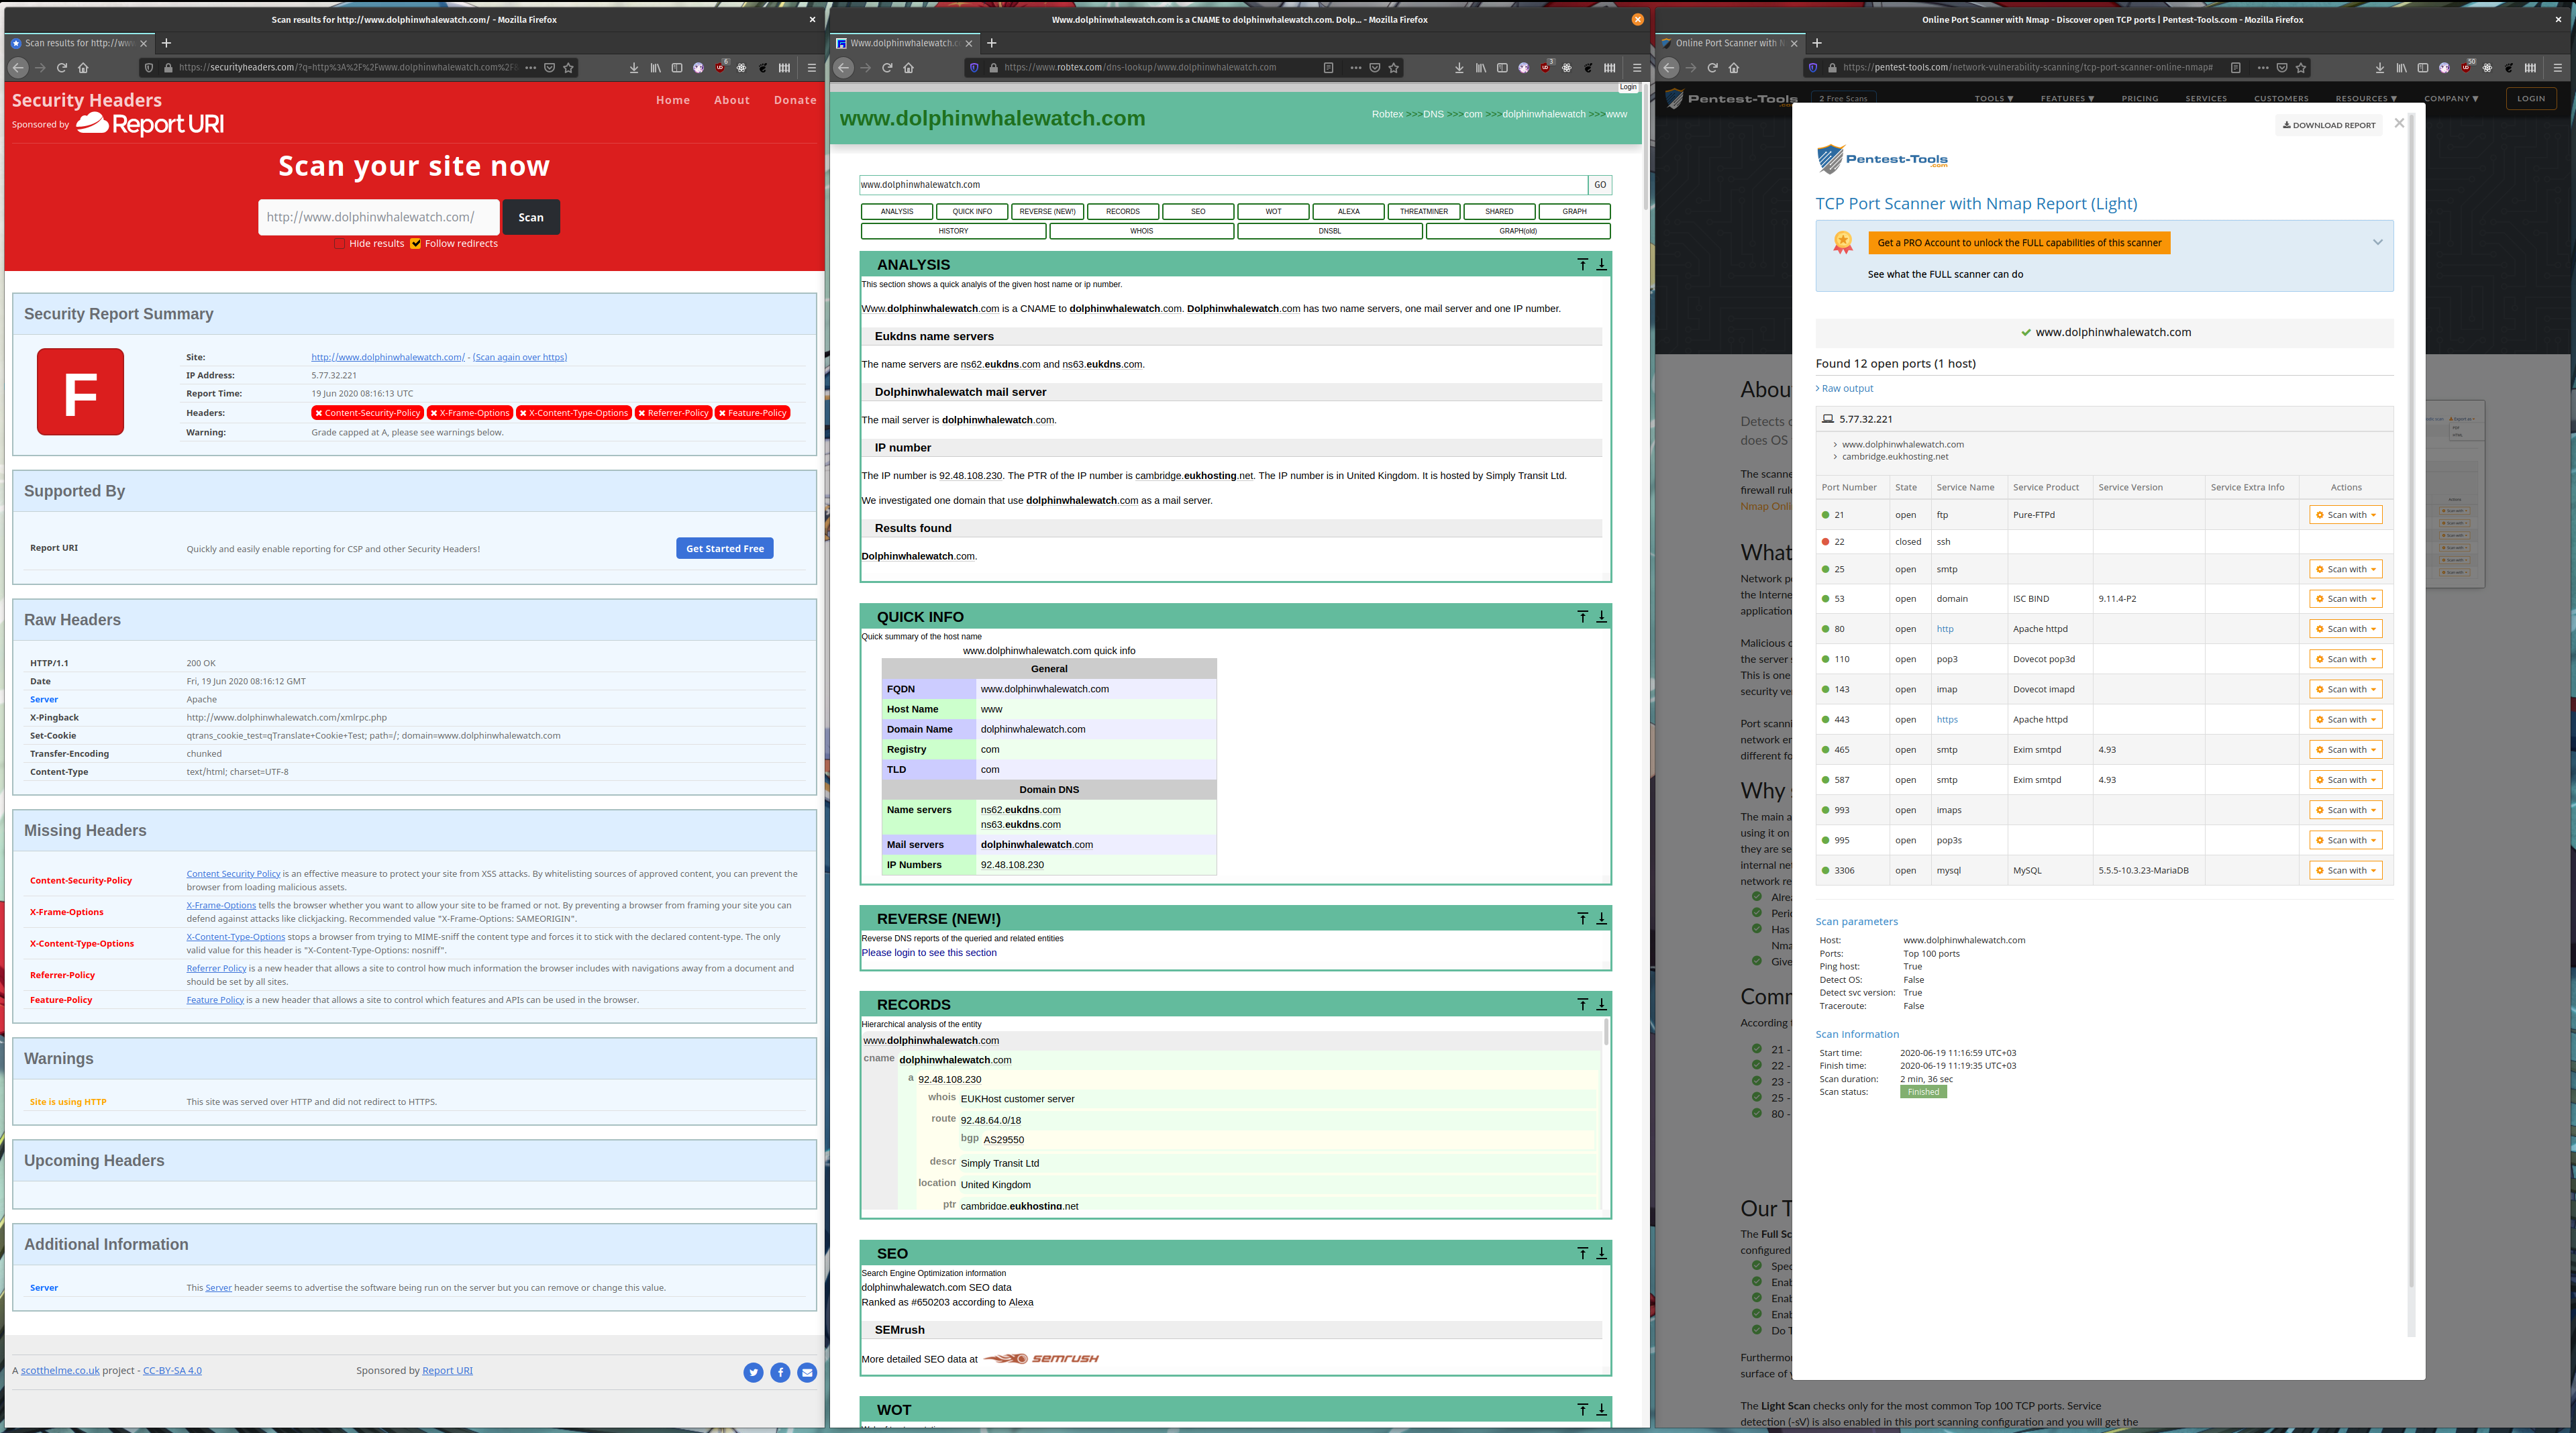
\includegraphics[width=.80\textwidth]{images/tooling.png}
\caption{Ejemplos de las ejecuciones de las herramientas.}
\label{FIG:tooling}
\end{figure}

\subsubsection{TCP Port scan}
Realiza un escaneo de puertos identico al que se puede realizar con NMap, con la diferencia que este entrega un agradable informe (el cual sirve para convencer a tu jefe que necesita cerrar sus puertos).

\subsubsection{Robtex}
Entrega información de caracter general del sitio, por ejemplo, puntaje de Alexa, registros DNS asociados, IPs conocidas.

\subsubsection{Security Headers}
Entrega un bonito reporte respecto a las cabeceras del sitio, las cuales dependiendo de como están configuradas pueden filtrar información del sistema o bien permitir ciertos ataques (CSFR-like).
\newline

Normalmente uno podría pensar que estas herramientas hacen exactamente lo mismo que hace cualquier herramienta disponible en una distribución de pentesting. Sin embargo, estas herramientas tienen el plus de que son ejecutadas fuera del entorno de la máquina, lo cual lo vuelve un poco mas realista cuando se trata de detectar intrusiones o amenazas provenientes de exponer el sitio a internet.

\begin{thebibliography}{9}
	\bibitem{REF:wpscan}
	WPScan
	\textit{WebSite}.
	https://wpscan.org/

	\bibitem{REF:self}
	Mi repositorio (donde están los comandos del laboratorio anterior)
	\textit{GitHub Repository}.
	https://github.com/KukyNekoi/UTAL/tree/master/ComputerScience/(2020-1)-Information_Security/Laboratorio%203
\end{thebibliography}

\end{document}